



\chapter{Einleitung}
    
    \begin{center}
        \begin{figure}[h]
            
\includegraphics[width=\textwidth]{img/PIA23645_PaleBlueDotRevisited_1600.jpg}
            \caption{``The Pale Blue Dot'' Feb. 14, 1990, by NASA\footnotemark.}
            \vspace{-6mm}
            \label{fig:my_label}
        \end{figure}
        \footnotetext{\fullcite{nasa.bluedot}}
    \end{center}
    
    ''Ein Bild sagt mehr aus als tausend Worte.`` Dieses bekannte Sprichwort drückt aus, wie mächtig Bilder als Kommunikationsmittel sind. 
    Bilder beinhalten Informationen, vermitteln Emotionen, erzählen Geschichten und sind ein Fenster in die Vergangenheit. 
    Bilder sind in der modernen Gesellschaft omnipräsent und im Alltag digital als auch analog unentbehrlich.
    Bilder unterscheiden sich je nach Aufnahme in den verschiedenen Eigenschaften ihrer Speicherung und Darstellung. 
    Zwei dieser Eigenschaften sind die Größe und die Auflösung eines Bildes. 
    Die Größe eines digitalen Bildes gibt an, wie viele Pixel es enthält, während die Auflösung eines Bildes angibt, wie viele Pixel pro Flächeneinheit vorhanden sind \ac{PPI}.

    ~

    Die Größe und die Auflösung eines Bildes haben Einfluss auf seine Qualität und seinen Speicherplatzbedarf.
    Um ein Bild für einen bestimmten Zweck zu nutzen, muss es häufig in seiner Größe und oder Auflösung verändert werden.
    Der Vorgang zur Veränderung der Größe und Auflösung wird als Bildskalierung bezeichnet\footfullcite{techlib.scaling}\footfullcite{abcdef.scaling} und ist eine grundlegende Operation in der digitalen Bildverarbeitung.
    Bildskalierung ist eine grundlegende Methode der Bildverarbeitung. Bildskalierung erlaubt die Änderung der Größe eines digitalen Bildes.
    Eine Gute Bildskalierung misst sich an ihren Eigenschaften in den Bereichen Rechenaufwand und Qualitätsverlust.
    Besonders wichtig ist der Qualitätsverlust, wenn man Bilder größer skaliert.
    Ein geeignetes Modell um diesen Prozess zu erklären ist das übertragen einer Zeichnung von einem kleinen Papier auf eine große Leinwand.
    Wird die Zeichnung lediglich unbedacht vergrößert, wird diese unscharf und verliert an Details.
    Das Ziel einer guten Bildskalierung ist es, diesen Effekt zu verhindern und die Zeichnung größenunabhängig scharf und detailreich darzustellen.

    ~

    Es gibt viele verschiedene Methoden, um die Größe eines Bildes zu ändern.
    Klassische Methoden verwenden Interpolationstechniken, die neue Pixel aus den vorhandenen Pixeln berechnen.
    Diese Methoden sind schnell und stellen einen geringen Rechenaufwand in Kombination mit geringer Komplexität dar.
    Jedoch kommt es mit diesen Algorithmen oft zu Qualitätsverlusten oder der Erzeugung von Artefakten.
    Moderne Anwendungen zur Skalierung von Bildern verwenden Deep-Learning-Techniken wie Convolutional Neural Networks \ac{CNN} oder Generative Adversarial Networks \ac{GAN}, die neue Pixel aus einem trainierten Modell erzeugen.
    Diese neuen Methoden sind komplex und benötigen mehr Rechenaufwand, können allerdings die Qualität des Bildes verbessern oder kreative Effekte erstellen.

    \begin{figure}[h!]
        \vspace{8mm}
        \centering
        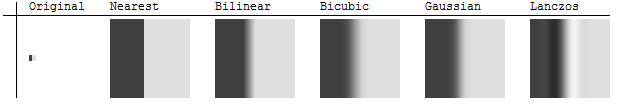
\includegraphics{img/xaR8r.png}
        \caption{Verschiedene Beispiele von upscaling Algorithmen\cite{whuber.lanczos}.}
        \label{fig:my_label}
        \vspace{4mm}
    \end{figure}

    Die Bildskalierung hat heute viele Anwendungen in verschiedenen Bereichen wie beispielweise Webdesign, Fotografie, Druck oder Videotechnik.
    Es gibt auch in modernen Anwendungen verschiedene Arten von Skalierungsverfahren, die sich in ihrer Funktionsweise und ihrem Ergebnis unterscheiden.
    Diese Arbeit schafft einen Überblick über klassische und moderne Skalierungsverfahren sowie deren ihre Vor- und Nachteile.
    Diese werden anhand von Beispielen inszeniert.
    Zuletzt wird basierend auf der Evaluierung der verschiedenen Verfahren eine Empfehlung für die beste Skalierungsmethode für verschiedene Bildtypen gegeben.

    ~

    In dieser Studienarbeit wird das zentrale Anliegen verfolgt mittels einer akribischen Untersuchung das optimale Gleichgewicht zwischen Komplexität, Rechenaufwand und Resultaten zu ermitteln. 
    Darüber hinaus erfolgt eine umfassende Erläuterung der Bewertungskriterien, die bei der Evaluierung solcher Verfahren Anwendung finden. 
    Das Firschungsvorhaben fokussiert sich auf die systematische Analyse unterschiedlicher Verfahren zur Skalierung von Bildern, um eine eine fundierte Empfehlung hinsichtlich der optimalen Methode abzugeben. 
    Die Berücksichtigung von Aspekten wie Algorithmuskomplexität, Rechenressourcen und erzielten Ergebnissen ist dabei von essenzieller Bedeutung. 
    Ferner werden präzise Kriterien erörtert, die zur objektiven Bewertung und Vergleichbarkeit der verschiedenen Skalierungsmethoden herangezogen werden können.
    Diese Studienarbeit strebt an, durch eine methodische Herangehensweise das Potenzial verschiedener Bildskalierungsmethoden zu evaluieren, um eine optimale Lösung zu finden, die ein ausgewogenes Verhältnis zwischen algorithmischer Komplexität, Ressourcenverbrauch und qualitativen Resultaten bietet. 
    Zusätzlich wird eine umfassende Beschreibung der Kriterien angestrebt, welche zur Beurteilung und Vergleichbarkeit dieser Methoden genutzt werden können.
    Hierzu werden zuerst die wichtigsten Konzepte der digitalen Bildverarbeitung und der Skalierung von Bildern erklärt und einige Beispiele für ihre Anwendung aufgezeigt. 
    Danach werden die traditionellen Skalierungsmethoden vorgestellt und  ihre Stärken sowie Schwächen verglichen. 
    Anschließend evaluiert diese Arbeit die neueren Skalierungsmethoden und vergleicht ihre Stärken sowie Schwächen. 
    Abschließend bewertet diese Studienarbeit die verschiedenen Methoden mit verschiedenen Maßstäben für die Bildqualität und gibt eine Empfehlung für die Auswahl einer passenden Methode. 
    Die Arbeit fasst sämtliche in ihr erarbeiteten Ergebnisse zusammen und bespricht deren Bedeutung bezüglich Möglichkeiten und Einschränkungen.
%----------------------
    \newpage
